  \documentclass{article}

\usepackage{textcomp}
\usepackage{enumitem}
\usepackage{soul}
\usepackage{tikz}
\usepackage{amsmath}
\usepackage{algorithm}
\usepackage{algpseudocode}
\setlistdepth{9}

\newlist{myEnumerate}{enumerate}{9}
\setlist[myEnumerate,1]{label=(\arabic*)}
\setlist[myEnumerate,2]{label=(\Roman*)}
\setlist[myEnumerate,3]{label=(\Alph*)}
\setlist[myEnumerate,4]{label=(\roman*)}
\setlist[myEnumerate,5]{label=(\alph*)}
\setlist[myEnumerate,6]{label=(\arabic*)}
\setlist[myEnumerate,7]{label=(\Roman*)}
\setlist[myEnumerate,8]{label=(\Alph*)}
\setlist[myEnumerate,9]{label=(\roman*)}
\begin{document}
\begin{figure}[t!]
\begin{center}
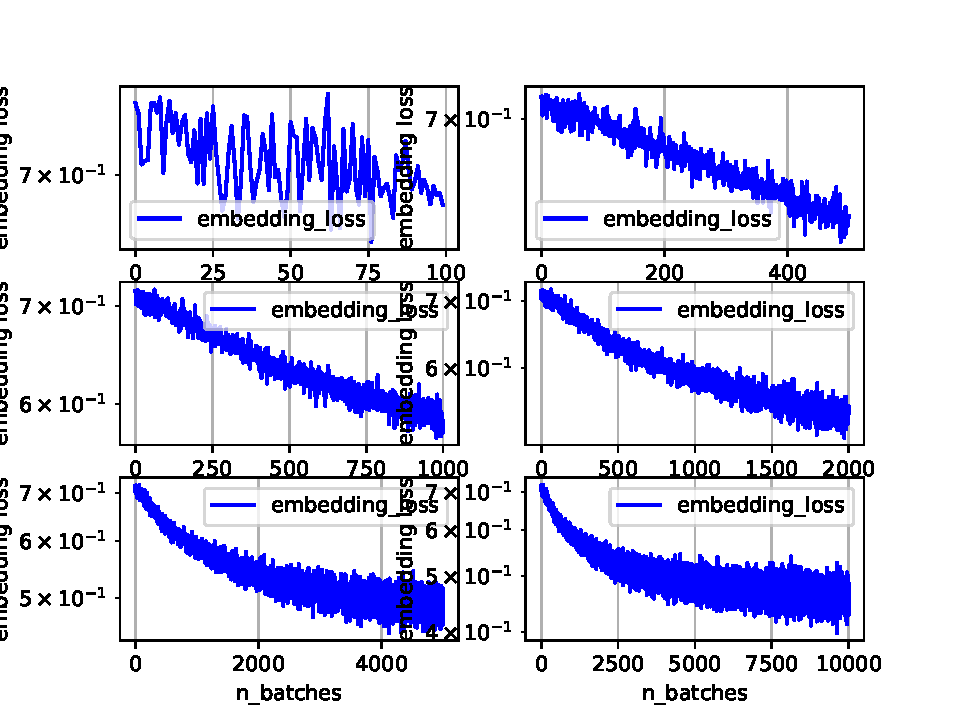
\includegraphics[width=1\textwidth]{figures/ml100k/embedding_loss_multipleplots.pdf}  
\end{center}
\caption{ml100k embedding loss with fixed alpha = 1.0}
\label{fig:ProperCover}
\end{figure}

\begin{figure}[t!]
\begin{center}
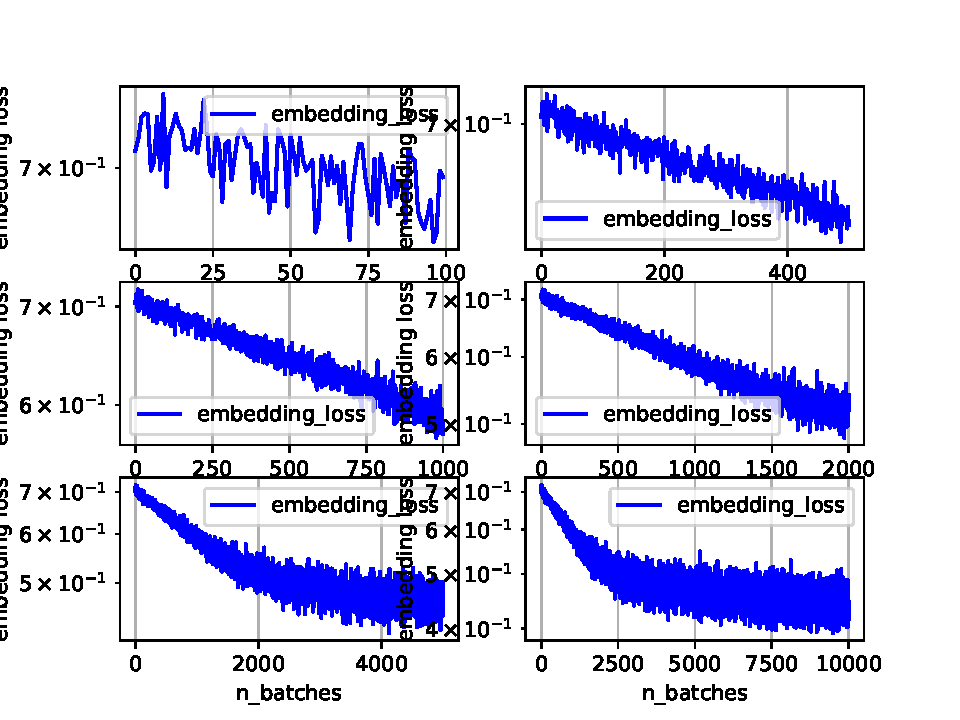
\includegraphics[width=1\textwidth]{figures/ml100k/embedding_loss_inc_alpha.pdf}  
\end{center}
\caption{ml100k embedding loss with increasing alpha. embedding loss does not seem to have converged}
\label{fig:ProperCover}
\end{figure}

\begin{figure}[t!]
\begin{center}
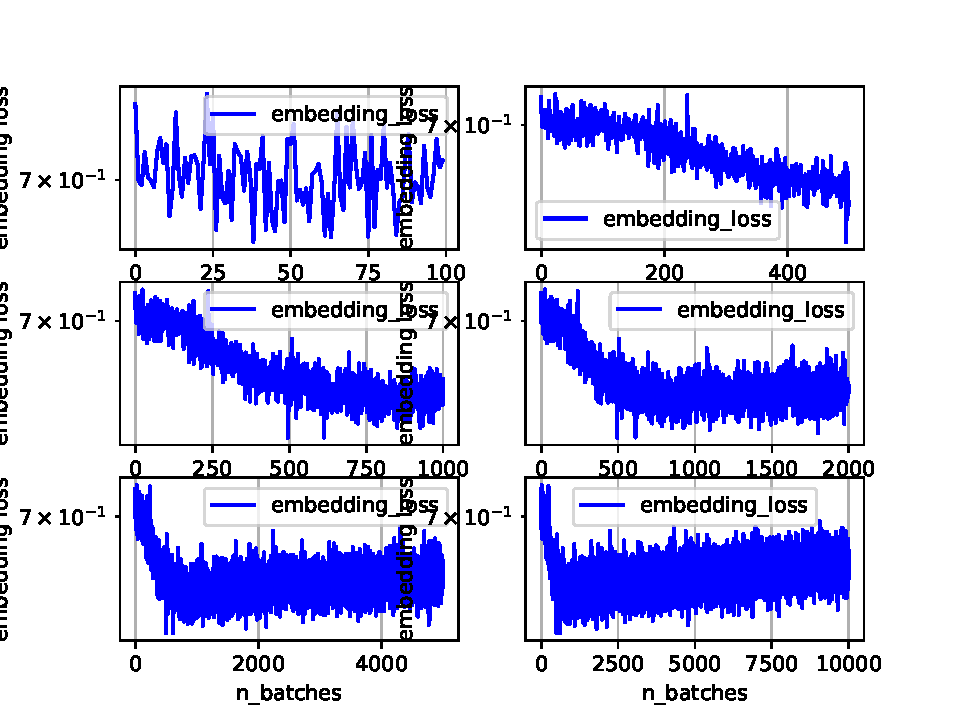
\includegraphics[width=1\textwidth]{figures/ml100k/embedding_loss_dec_alpha.pdf}  
\end{center}
\caption{ml100k embedding loss with decreasing alpha.}
\label{fig:ProperCover}
\end{figure}

\begin{figure}[t!]
\begin{center}
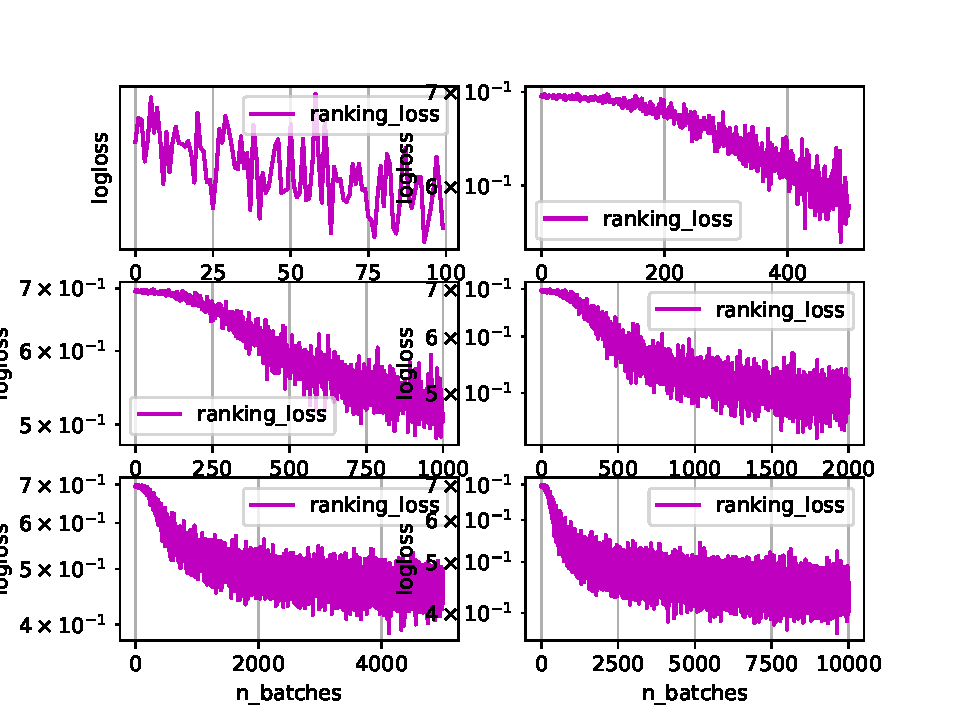
\includegraphics[width=1\textwidth]{figures/ml100k/ranking_loss_multipleplots.pdf}  
\end{center}
\caption{ml100k ranking loss with fixed alpha = 1.0}
\label{fig:ProperCover}
\end{figure}

\begin{figure}[t!]
\begin{center}
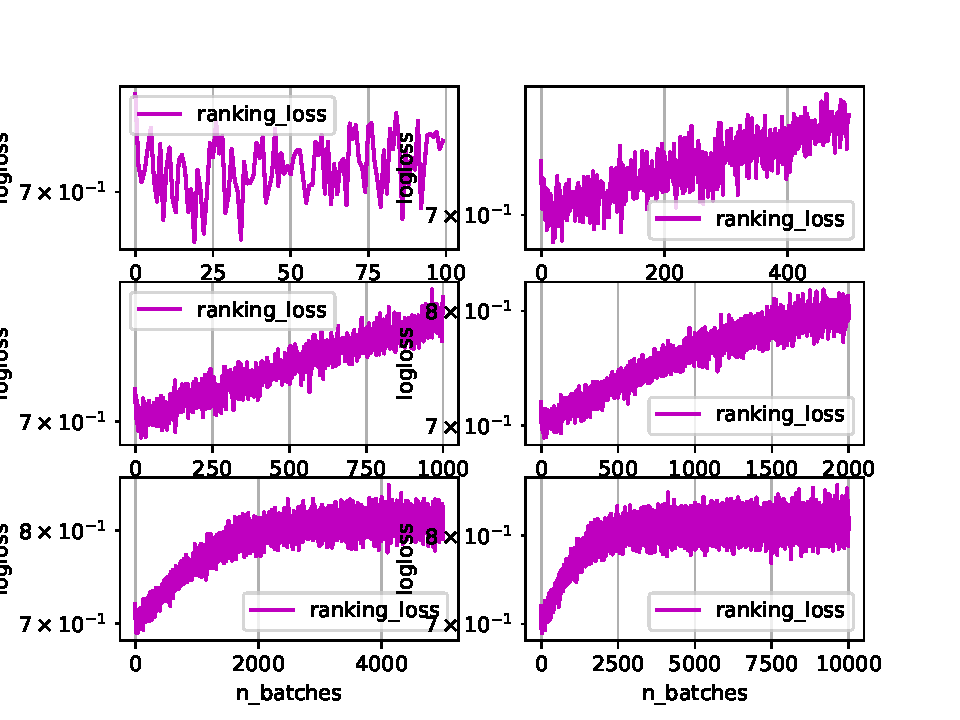
\includegraphics[width=1\textwidth]{figures/ml100k/ranking_loss_inc_alpha.pdf}  
\end{center}
\caption{ml100k ranking loss with increasing alpha. ranking loss does not seem to have converged}
\label{fig:ProperCover}
\end{figure}

\begin{figure}[t!]
\begin{center}
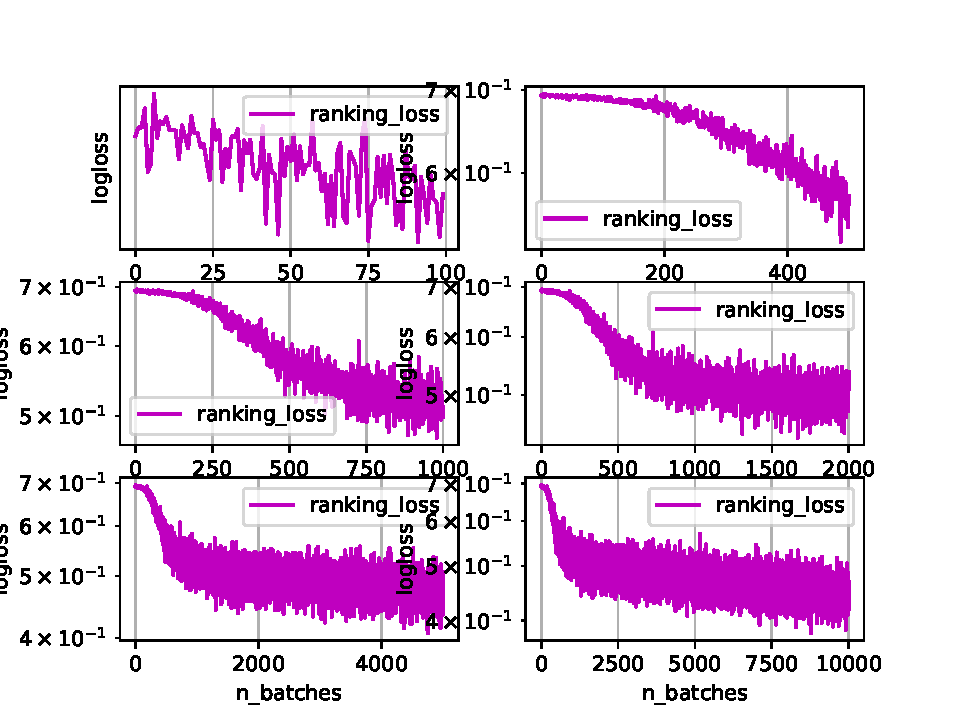
\includegraphics[width=1\textwidth]{figures/ml100k/ranking_loss_dec_alpha.pdf}  
\end{center}
\caption{ml100k ranking loss with decreasing alpha.}
\label{fig:ProperCover}
\end{figure}

\begin{figure}[t!]
\begin{center}
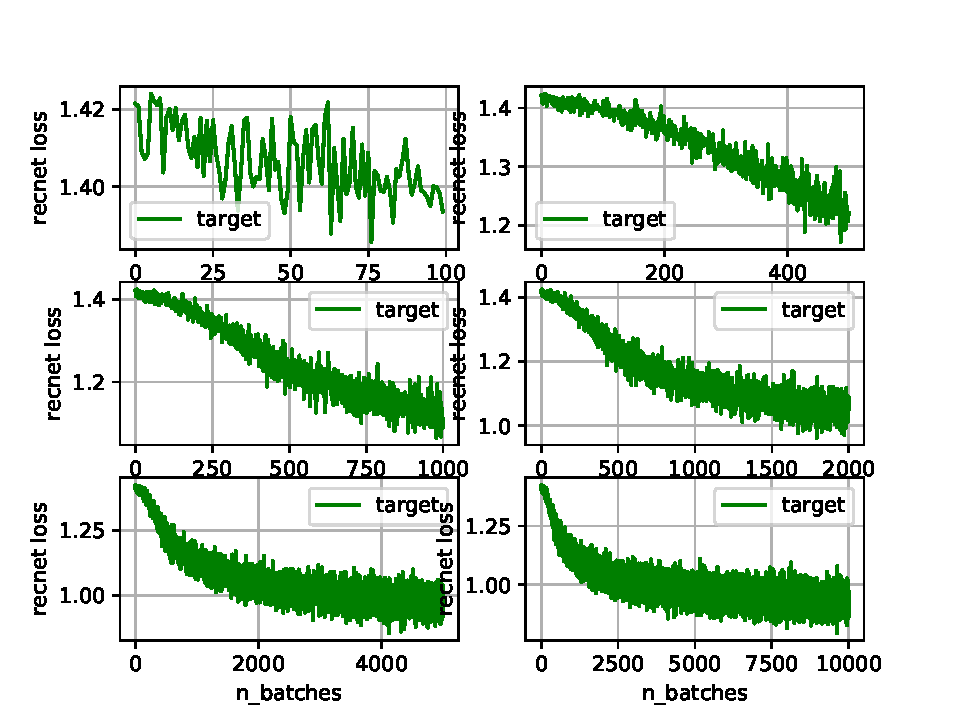
\includegraphics[width=1\textwidth]{figures/ml100k/target_loss_multipleplots.pdf}  
\end{center}
\caption{ml100k target loss with fixed alpha = 1.0}
\label{fig:ProperCover}
\end{figure}

\begin{figure}[t!]
\begin{center}
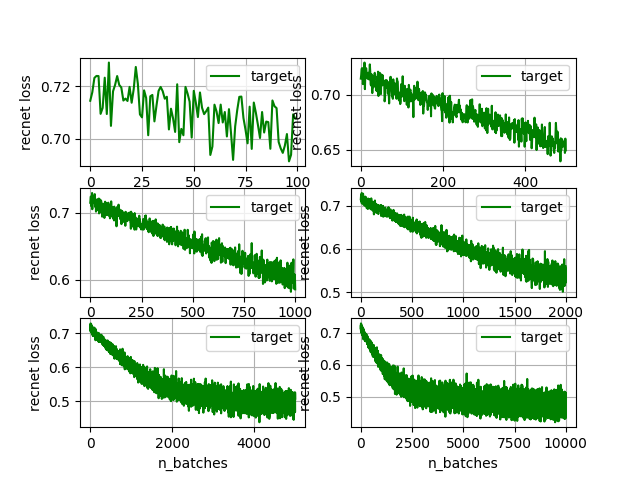
\includegraphics[width=1\textwidth]{figures/ml100k/target_loss_inc_alpha}  
\end{center}
\caption{ml100k target loss with increasing alpha. target loss does not seem to have converged}
\label{fig:ProperCover}
\end{figure}

\begin{figure}[t!]
\begin{center}
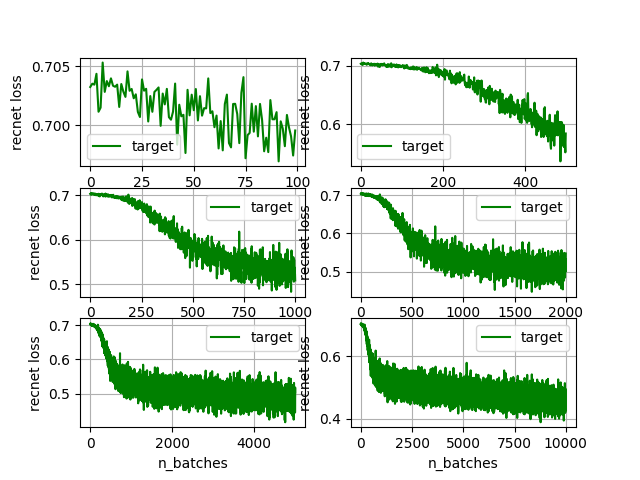
\includegraphics[width=1\textwidth]{figures/ml100k/target_loss_dec_alpha}  
\end{center}
\caption{ml100k target loss with decreasing alpha.}
\label{fig:ProperCover}
\end{figure}

\begin{table}[]
\centering
\caption{Results obtained on ML-100K. Settings with fixed $\alpha$, increasing $\alpha$ and decreasing $\alpha$}
\label{my-label}
\begin{tabular}{|c|c|c|c|}
\hline
                              & MAP@1 & MAP@5 & MAP@10 \\ \hline
$\alpha$ = 1.0, $\beta$ = 0.1 & 0.888 & 0.865 & 0.842  \\ \hline
Increase $\alpha$             &   0.819    &0.804       &   0.775     \\ \hline
Decrease $\alpha$             &   0.8375    &0.822       & 0.794       \\ \hline
\end{tabular}
\end{table}



\end{document}
